\documentclass[10pt,a4paper,notitlepage]{article}
\usepackage[utf8]{inputenc}
\usepackage{amsmath}
\usepackage{amsfonts}
\usepackage{amssymb}
\usepackage{fullpage}
\usepackage{lastpage}
\usepackage{lscape}
\usepackage{dsfont}
\usepackage{fancyhdr}
\usepackage{multirow}
\usepackage{booktabs}
\usepackage{bm}
\usepackage{fancyvrb}
\usepackage{xcolor}
\usepackage{tikz}
\usetikzlibrary{automata, positioning, arrows}
\usepackage{graphicx}
\graphicspath{{./Graphics/}}
\usepackage{float}
\usepackage{nameref}
\usepackage[backend=bibtex,style=authortitle-ibid]{biblatex}
\usepackage{diagbox}
\addbibresource{References.bib}



\pagestyle{fancy}
\fancyhf{}
\renewcommand{\headrulewidth}{0pt}
\cfoot{Page \thepage\ of \pageref{LastPage}}

\newcommand{\abs}[1]{\lvert#1\rvert}
\newcommand{\Z}{\mathbb{Z}}
\newcommand{\Q}{\mathbb{Q}}
\newcommand{\C}{\mathbb{C}}
\newcommand{\N}{\mathbb{N}}
\newcommand{\R}{\mathbb{R}}

\newcommand{\p}{\mathbb{P}}
\newcommand{\E}{\mathbb{E}}
\newcommand{\Var}{\text{Var}}

\newcommand{\x}{\mathbf{x}}
\newcommand{\y}{\mathbf{y}}
\newcommand{\X}{\mathbf{X}}

\begin{document}
\begin{titlepage}
	\centering
	\vspace*{5cm}
	{\large{University of Cambridge} \par}
	\vspace{1cm}
	{\Large \textsc{Part II CATAM Project}\par}
	\vspace{1.5cm}
	{\huge\bfseries Markov Chain Monte Carlo\par}
	\vspace{2cm}
	{\Large Jonah M. Gibbon\\ \vspace{0.6cm} April, 2022}
	\vfill
	


% Bottom of the page
	{Submitted in the fulfilment of the Mathematical Tripos, Part II.}
\end{titlepage}
\subsection*{\centering Question 1}
For the sake of notation, let $x_{i:j}$ denote $(x_{i},x_{i+1},\hdots,x_{j})$. Then
\begin{equation}
\begin{aligned}\label{eq:1}
\sum_{\x}\pi(\x)\pi(\x,\y) &= \sum_{\x}\pi(x_{1}|x_{2:m})\pi(x_{2:m})\cdot \prod_{k=1}^{m}\pi(y_{k}|y_{1:k-1},x_{k+1:m})
\end{aligned}
\end{equation}
We now use the identity
\begin{equation}\label{eq:2}
\p(X|Y,Z)=\frac{\p(X,Y,Z)}{\p(Y,Z)}=\frac{\p(Z|X,Y)\p(X,Y)}{\p(Z|Y)\p(Y)}=\frac{\p(Z|X,Y)\p(X|Y)}{\p(Z|Y)}
\end{equation}
Setting $X=y_{k}$, $Y=y_{1:k-1}$ and $Z=x_{k+1:m}$, this transforms equation \eqref{eq:1} to
\begin{equation}
\begin{aligned}
&\sum_{\x}\pi(x_{1}|x_{2:m})\pi(x_{2:m})\cdot \prod_{k=1}^{m}\frac{\pi(x_{k+1:m}|y_{1:k})\pi(y_{k}|y_{1:k-1})}{\pi(x_{k+1:m}|y_{1:k-1})}\\
= &\prod_{k=1}^{m}\left\{(\pi(y_{k}|y_{1:k-1})\right\}\sum_{\x}\left\{\pi(x_{1}|x_{2:m})\pi(x_{2:m})\prod_{k=1}^{m-1}\frac{\pi(x_{k+1:m}|y_{1:k})}{\pi(x_{k+1:m}|y_{1:k-1})}\right\}
\end{aligned}
\end{equation}
However we notice that
\begin{equation}
\begin{aligned}
&\sum_{\x}\left\{\pi(x_{1}|x_{2:m})\pi(x_{2:m})\prod_{k=1}^{m-1}\frac{\pi(x_{k+1:m}|y_{1:k})}{\pi(x_{k+1:m}|y_{1:k-1})}\right\}\\ 
= &\sum_{\x}\pi(x_{1}|x_{2:m})\pi(x_{2:m})\frac{\pi(x_{2:m}|y_{1})}{\pi(x_{2:m})}\cdot \frac{\pi(x_{3:m}|y_{1:2})}{\pi(x_{3:m}|y_{1})}\, \cdots\, \frac{\pi(x_{m}|y_{1:m-1})}{\pi(x_{m}|y_{1:m-2})}\\
= &\sum_{\x}\pi(x_{1}|x_{2:m})\pi(x_{m}|y_{1:m-1})\prod_{k=1}^{m-2}\frac{\pi(x_{k+1:m}|y_{1:k})}{\pi(x_{k+2:m}|y_{1:k})}\\
\end{aligned}
\end{equation}
Notice that $x_{1}$ only appears in the first factor, so by summing over $x_{1}$ it disappears. Then notice the only place $x_{2}$ occurs is in $\pi(x_{2:m}|y_{1})$, so by summing over $x_{2}$ this turns into $\pi(x_{3:m}|y_{1})$ cancelling with the denominator. Proceeding by induction we claim that the above is equal to 1. We therefore conclude that
\begin{equation}
\sum_{\x}\pi(\x)\pi(\x,\y)=\prod_{k=1}^{m}\pi(y_{k}|y_{1:k-1})=\pi(\y)
\end{equation}
and hence $\pi$ is an invariant measure of this Markov chain.
\subsection*{\centering Question 2}
Using the identity in equation \eqref{eq:2} we deduce that $\pi(\mu_{k}|\bm{\mu}_{-k},\theta,\bm{\sigma}^{2},\y)\propto \pi(\y|\bm{\mu},\theta,\bm{\sigma}^{2})\pi(\mu_{k}|\bm{\mu}_{-k},\theta,\bm{\sigma}^{2})=\pi(\y|\bm{\mu},\theta,\bm{\sigma}^{2})\pi(\mu_{k}|\theta)$.
Hence the posterior distribution of $\mu_{k}$ is proportional to
\begin{equation}
\begin{aligned}
&\prod_{l=1}^{K}\prod_{t=1}^{T}\left\{\frac{1}{\sqrt{2\pi \sigma_{l}^{2}}}\exp\left(-\frac{1}{2\sigma_{l}^{2}}\left(y_{lt}-\mu_{l}\right)^{2}\right)\right\}\frac{1}{\sqrt{2\pi\sigma_{0}^{2}}}\exp\left(-\frac{1}{2\sigma_{0}^{2}}\left(\mu_{k}-\theta\right)^{2}\right)\\
\propto &\prod_{t=1}^{T}\exp\left(-\frac{1}{2\sigma_{k}^{2}}\left(y_{kt}-\mu_{k}\right)^{2}\right)\exp\left(-\frac{1}{2\sigma_{0}^{2}}\left(\mu_{k}-\theta\right)^{2}\right)\\
\propto &\exp\left(\left(-\frac{T}{2\sigma_{k}^{2}}-\frac{1}{2\sigma_{0}^{2}}\right)\mu_{k}^{2}+\left(\frac{1}{\sigma_{k}^{2}}\sum_{t=1}^{T}y_{kt}+\frac{\theta}{\sigma_{0}^{2}}\right)\mu_{k}\right)\\
\propto &\exp\left(-\frac{T\sigma_{k}^{-2}+\sigma_{0}^{-2}}{2}\left(\mu_{k}-\frac{\sigma_{k}^{-2}\sum_{t=1}^{T}y_{kt}+\theta\sigma_{0}^{-2}}{T\sigma_{k}^{-2}+\sigma_{0}^{-2}}\right)^{2}\right)
\end{aligned}
\end{equation}
Notice that this is proportional to a normal distribution with the required parameters in the project booklet. An almost identical procedure is used for the second result, since $\pi(\theta |\bm{\sigma}^{2},\bm{\mu},\y)\propto \pi(\y|\bm{\mu},\bm{\sigma}^{2},\theta)\pi(\theta|\bm{\mu},\bm{\sigma}^{2})\propto\pi(\bm{\mu}|\theta)\pi(\theta)$. Hence taking the product over $k$ and interchanging the parameters

\begin{equation}
\begin{aligned}
\sigma_{k}^{-2} &\mapsto \sigma_{0}^{-2}\\
\sigma_{0}^{-2} &\mapsto \tau_{0}^{-2}\\
\y_{kt} &\mapsto \mu_{k}\\
\theta &\mapsto \mu_{0}\\
\end{aligned}
\end{equation}
we derive the second distribution.
For the final result, we know that the distribution $\pi(\sigma_{k}^{-2}|\bm{\mu},\theta,\bm{\sigma}^{2}_{-k},\y)\propto \pi(\y|\bm{\mu},\theta,\bm{\sigma}^{2})\pi(\sigma_{k}^{-2}|\bm{\mu},\theta,\bm{\sigma}^{2}_{-k})=\pi(\y|\bm{\mu},\theta,\bm{\sigma}^{2})\pi(\sigma_{k}^{-2})$. So the posterior distribution is proportional to
\begin{equation}
\begin{aligned}
&\prod_{l=1}^{K}\prod_{t=1}^{T}\left\{\frac{1}{\sqrt{2\pi \sigma_{l}^{2}}}\exp\left(-\frac{1}{2\sigma_{l}^{2}}\left(y_{lt}-\mu_{l}\right)^{2}\right)\right\}\cdot \frac{\left(\sigma_{k}^{-2}\right)^{\alpha_{0}-1}\exp\left(-\beta_{0}\sigma_{k}^{-2}\right)\beta_{0}^{\alpha_{0}}}{\Gamma\left(\alpha_{0}\right)}\\
\propto &\left(\sigma_{k}^{-2}\right)^{T/2}\exp\left(-\frac{1}{2}\sigma_{k}^{-2}\sum_{t=1}^{T}\left(y_{kt}-\mu_{k}\right)^{2}\right)\left(\sigma_{k}^{-2}\right)^{\alpha_{0}-1}\exp\left(-\beta_{0}\sigma_{k}^{-2}\right)\\
= &\left(\sigma_{k}^{-2}\right)^{\alpha_{0}+T/2-1}\exp\left(-\left(\beta_{0}+\frac{1}{2}\sum_{t=1}^{T}\left(y_{kt}-\mu_{k}\right)^{2}\right)\sigma_{k}^{-2}\right)
\end{aligned}
\end{equation}
This is proportional to the Gamma distribution with the same parameters given in the project booklet, and hence we're done.
The marginal prior distribution for $\pi(\mu_{k})=\int_{-\infty}^{+\infty}\pi(\mu_{k}|\theta)\pi(\theta)d\theta$. We can calculate this as
\begin{equation}
\begin{aligned}
\pi(\mu_{k}) &\propto \int_{-\infty}^{+\infty}\exp\left(-\frac{1}{2\sigma_{0}^{2}}\left(\theta-\mu_{k}\right)^{2}\right)\exp\left(-\frac{1}{2\tau_{0}^{2}}\left(\theta-\mu_{0}\right)^{2}\right)d\theta\\
&\propto \exp\left(-\frac{1}{2\tau_{0}^{2}+2\sigma_{0}^{2}}\left(\mu_{k}-\mu_{0}\right)^{2}\right)\\
\end{aligned}
\end{equation}
From this we conclude that the marginal prior for $\mu_{k}$ is distributed as such
\begin{equation}
\pi\left(\mu_{k}\right)\sim \text{N}\left(\mu_{0},\tau_{0}^{2}+\sigma_{0}^{2}\right)
\end{equation}
\subsection*{\centering Question 3}
The code named \nameref{cd:Gibbs}, referenced on page \pageref{cd:Gibbs}, was used to sample from the posterior distribution using the described MCMC method.\footnote{The function \texttt{Gibbs} and the object \texttt{Data} will be used implicitly throughout the rest of this project, and wont be included in any subsequent referencing.} The test data below in Table \ref{tb:6} is a small section of output from the first 5 iterations.
\begin{table}[H]
\centering
\begin{tabular}{c|cccccc}
& $\x^{0}$ & $\x^{1}$ & $\x^{2}$ & $\x^{3}$ & $\x^{4}$ & $\x^{5}$\\ \hline
$\mu_{1}$ & 60.0 & 77.810272 & 84.941201 & 84.404838 & 82.554353 & 84.320647\\ 
$\mu_{2}$ & 60.0 & 53.986773 & 61.205653 & 50.919007 & 47.719512 & 55.28883\\ 
$\mu_{3}$ & 60.0 & 54.46738 & 52.862724 & 49.288816 & 57.539684 & 47.780734\\ 
$\sigma_{1}^{2}$ & 100.0 & 82.554671 & 18.999169 & 105.86238 & 51.541417 & 27.141017\\ 
$\sigma_{2}^{2}$ & 100.0 & 157.20313 & 65.218544 & 25.098216 & 143.12897 & 79.378385\\ 
$\sigma_{3}^{2}$ & 100.0 & 48.066815 & 32.884554 & 78.324008 & 107.22865 & 159.2443\\ 
$\theta$ & 60.0 & 66.303817 & 55.594835 & 57.2068 & 60.967041 & 58.96342
\end{tabular}
\caption{Test Data for Gibbs Sampler}\label{tb:6}
\end{table}

The choice of parameters suggest that each team roughly scores 60 points per year, however $\sigma_{0}^{2}+\tau_{0}^{2}=500$, suggesting that there is roughly $\pm 2\sqrt{\sigma_{0}^{2}+\tau_{0}^{2}}=\pm 45$ uncertainty in the value of any teams mean $\mu_{k}$. We also note that initially $\E(\sigma_{k}^{2})=10^{-2}$, and $\Var(\sigma_{k}^{-2})=10$, suggesting that there is a large uncertainty in the data, with a small scope to change this uncertainty.

We aim to choose the initial state $\x^{0}$ as close to the prior distribution as possible. Assuming no knowledge of the observed data $\y$, it makes sense to set each of the values of the parameters to their expected value under the prior distribution. Hence $\mu_{k}^{0}=60$ and $\theta^{0}=60$. Note the value of $\E(\sigma_{k}^{2})$ is negative if we use the extended Gamma function for negative numbers which makes no sense, however using Jensen's inequality we deduce that $\E(\sigma_{k}^{2})\geq 100$, and so it has been set to 100.
\subsection*{\centering Question 4}
The posterior means of $(\theta,\mu_{k},\sigma_{k}^{2})$ were calculated using $N=250$ samples by \nameref{cd:3}, referenced on page \pageref{cd:3}, as well as generating a histogram for $\pi(\theta |\y)$ using $N=10^{5}$. These are presented below in Table \ref{tb:1} and Figure \ref{fg:1}.
\begin{table}[H]
\centering
\begin{tabular}{c|cc|cc} 
$k$ & Estimated $\mu_{k}$ & Empirical $\mu_{k}$ & Estimated $\sigma^{2}$ & Empirical $\sigma^{2}$\\ \hline
1 & 81.496883 & 83.8 & 52.714064 & 22.7\\ 
2 & 52.13558 & 51.6 & 89.648396 & 39.3\\ 
3 & 50.672261 & 49.6 & 127.38336 & 62.8\\ 
4 & 52.508082 & 51.0 & 137.94752 & 76.0\\ 
5 & 48.138956 & 47.4 & 27.386959 & 13.3\\ 
6 & 69.784992 & 75.2 & 284.56201 & 154.2\\ 
7 & 51.63744 & 49.6 & 162.13317 & 96.8\\ 
8 & 48.756523 & 48.2 & 38.925028 & 18.2\\ 
9 & 62.29331 & 63.2 & 182.30559 & 101.2\\ 
10 & 74.386134 & 76.4 & 59.714628 & 21.8\\ 
11 & 49.838218 & 49.6 & 24.982545 & 13.8\\ 
12 & 59.952036 & 60.8 & 202.51054 & 121.7\\ 
13 & 48.286265 & 46.2 & 190.7173 & 78.7\\ 
14 & 51.535571 & 51.2 & 45.20259 & 25.7
\end{tabular}
\caption{Estimated Posterior Means of $\mu_{k}$ and $\sigma^{2}_{k}$}\label{tb:1}
\end{table}
\begin{figure}[H]
\centering
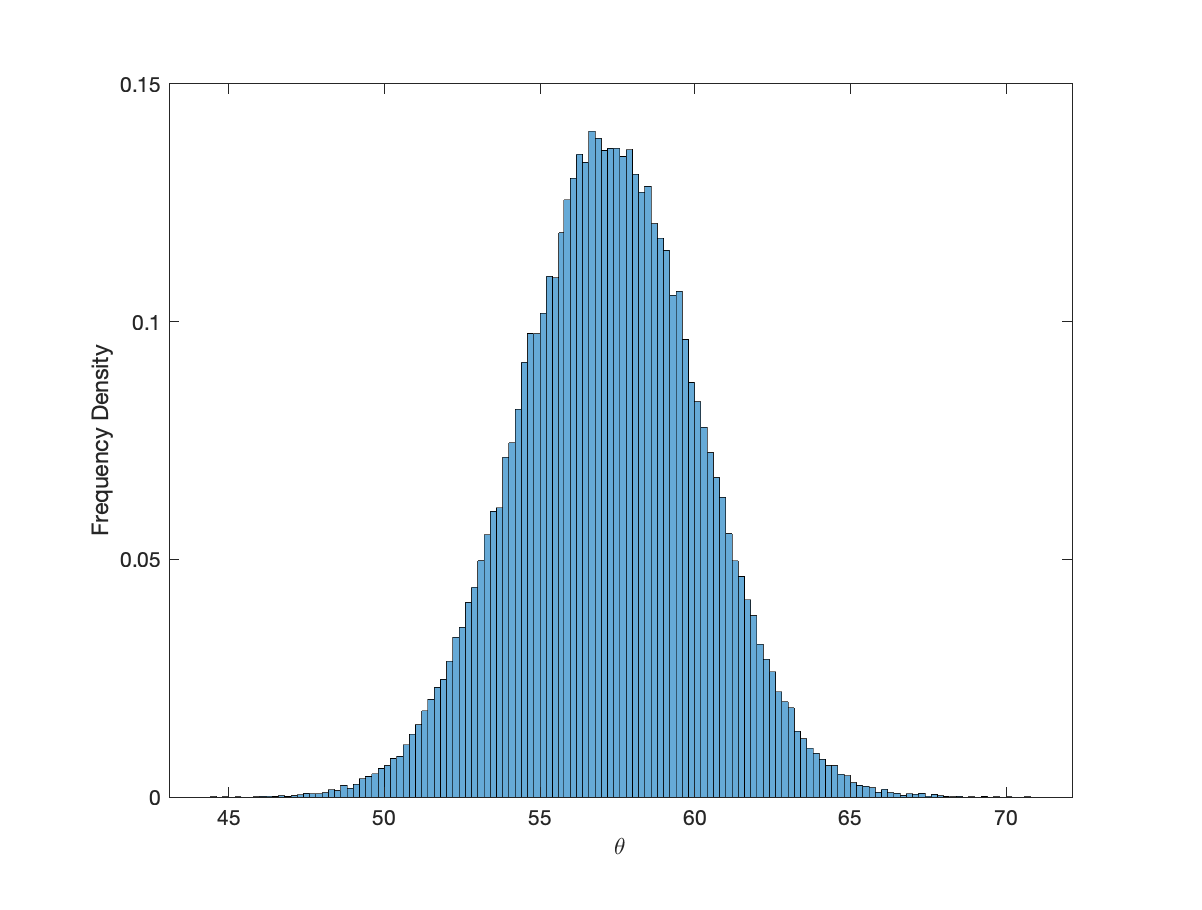
\includegraphics[width=13cm]{Image_1}
\caption{Posterior distribution of $\theta$}\label{fg:1}
\end{figure}
The empirical means and variances were calculated from the data $\y$ for comparison. We can see that the expected value of $\mu_{k}$ under the posterior distribution is very close to the average of the data, whereas the variance seems to remain significantly higher than the empirical variance (roughly double). This confirms the predictions in Question 3, that the large uncertainty in the data does not decrease with the observations $\y$.\\

The posterior mean of $\theta$ was calculated as 57.19, slightly less than the starting value 60. The distribution appears to be Gaussian. We can try to calculate this distribution analytically: 
\begin{equation}
\begin{aligned}
\pi(\theta|\y) &\propto \pi(\y|\theta)\pi(\theta)\\
&=\left(\int_{\bm{\mu},\bm{\sigma}^{-2}}\pi(\y|\bm{\mu},\bm{\sigma}^{-2},\theta)\pi(\bm{\mu},\bm{\sigma}^{-2}|\theta)\,\text{d}\bm{\mu}\,\text{d}\bm{\sigma}^{-2}\right)\pi(\theta)\\
&=\left(\int_{\bm{\mu},\bm{\sigma}^{-2}}\pi(\y|\bm{\mu},\bm{\sigma}^{-2})\pi(\bm{\mu}|\theta)\pi(\bm{\sigma}^{-2})\,\text{d}\bm{\mu}\,\text{d}\bm{\sigma}^{-2}\right)\pi(\theta)
\end{aligned}
\end{equation}
Firstly note that we may treat each value of $k$ independently and instead take the product over this at the end. We therefore can simplify the problem to calculating the above for some fixed value of $k$ (for the sake of simplicity drop the subscript).  We then calculate the bracketed part above as
\begin{equation}
\begin{aligned}
&\int_{-\infty}^{+\infty}\int_{0}^{\infty}\left(\sigma^{-2}\right)^{T/2+\alpha_{0}-1}\exp\left(-\frac{\sigma^{-2}}{2}\left(\sum_{i=1}^{T}\left(y_{ki}-\mu\right)^{2}\right)-\frac{1}{2\sigma_{0}^{2}}\left(\mu-\theta\right)^{2}-\beta_{0}\sigma^{-2}\right)\text{d}\sigma^{-2}\,\text{d}\mu\\
\propto &\int_{-\infty}^{\infty}\left(\frac{1}{\frac{1}{2}\sum_{i=1}^{T}\left(y_{ki}-\mu\right)^{2}+\beta_{0}}\right)^{T/2+\alpha_{0}}\exp\left(-\frac{1}{2\sigma_{0}^{2}}\left(\mu-\theta\right)^{2}\right)\text{d}\mu
\end{aligned}
\end{equation}
The values of $\alpha_{0}$ and $\beta_{0}$ can be ignored since they're comparably small. Modelling this function gives a very similar (though not exact) Gaussian distribution for $\theta$. Assuming it is, then by taking the product of $K+1$ Gaussian distributions it will indeed give a Gaussian,  and thus we conclude that the posterior distribution of $\theta$ is approximately (but not exactly) Gaussian.

\subsection*{\centering Question 5}
\nameref{cd:4}, referenced on page \pageref{cd:4}, was used to estimate $\p(\mu_{k}>\theta|\y)$ by finding the average of the indicator function $\mathds{1}_{\mu_{k}>\theta}$ over the posterior distribution. The results below in Table \ref{tb:2} were produced when $N=1000$.
\begin{table}[H]
\centering
\begin{tabular}{c|c} $k$&$\p(\mu_{k}>\theta|\y)$\\\hline 
1 & 1.000\\
2 & 0.104\\
3 & 0.100\\
4 & 0.152\\
5 & 0.004\\
6 & 0.932\\
7 & 0.120\\
8 & 0.004\\
9 & 0.840\\
10 & 0.996\\
11 & 0.036\\
12 & 0.728\\
13 & 0.056\\
14 & 0.076 \\
\end{tabular}
\caption{Estimated values of $\p(\mu_{k}>\theta|\y)$}\label{tb:2}
\end{table}
Notice how all of these probabilities are either very large or very small, there is not much uncertainty if a team is above or below average. This suggests that the variance in $\mu_{k}$ will be small, since then $\mu_{k}$ will either lie on one side or the other of $\theta$.

\subsection*{\centering Question 6}
The simulations in Questions 4-5 were repeated $500$ times with $N=250$ using \nameref{cd:4}, and the sample variances were calculated and tabulated below in Table \ref{tb:3}. 
\begin{table}[H]
\centering
\begin{tabular}{c|c|c}
$k$&S.V in $\mu_{k}$ & S.V in $\p(\mu_{k}>\theta|\y)$\\
\hline
1 & 0.31932168 & 1.9852249e-5\\
2 & 0.050576302 & 4.5196287e-4\\
3 & 0.073926224 & 3.4977321e-4\\
4 & 0.079487089 & 5.1195742e-4\\
5 & 0.025197288 & 3.1824032e-5\\
6 & 0.31273951 & 2.2441523e-4\\
7 & 0.11360919 & 5.2450315e-4\\
8 & 0.030712084 & 6.5253322e-5\\
9 & 0.098515333 & 6.3724319e-4\\
10 & 0.081711728 & 1.0228200e-5\\
11 & 0.020928080 & 9.9218212e-5\\
12 & 0.10951773 & 8.4340066e-4\\
13 & 0.11541775 & 2.3513036e-4\\
14 & 0.037308591 & 3.0127455e-4\\
\end{tabular}
\caption{Sample Variances in $\mu_{k}$ and $\p(\mu_{k}>\theta|\y)$}\label{tb:3}
\end{table}
Notice the sample variances in $\mu_{k}$ are indeed small, which causes the variance in $\p(\mu_{k}>\theta|\y)$ to be small, since $\mu_{k}$ will likely lie to one side or the other of $\theta$ (unless the two are very close). The sample variances of $\p(\mu_{k}>\theta|\y)$ is far smaller than those of $\mu_{k}$, and this is because the indicator function does not depend contentiously on the values of $\mu_{k}$ and $\theta$. Hence $\mathds{1}_{\mu_{k}>\theta}$ is roughly constant over the posterior distribution.

To investigate how this variance decays with $N$, the method above was repeated $500$ times with $N=20,30,50,100,150,250$ using \nameref{cd:4}. The sample variances were then normalised (sample variance at $N=20$ is 1) such that they could be compared when plotted in Figures \ref{fg:2} and \ref{fg:3} below.
\begin{figure}[H]
\centering
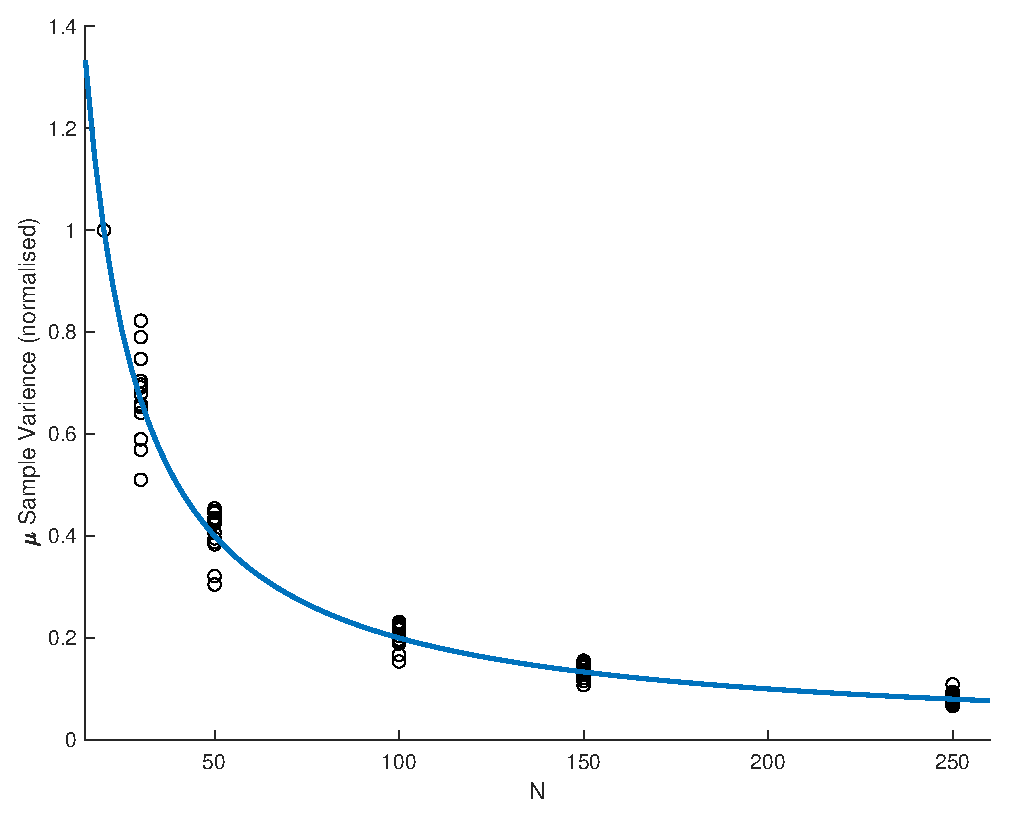
\includegraphics[width=12cm]{Image_2}
\caption{Sample variance of $\mu_{k}$ for different $N$}\label{fg:2}
\end{figure}

\begin{figure}[H]
\centering
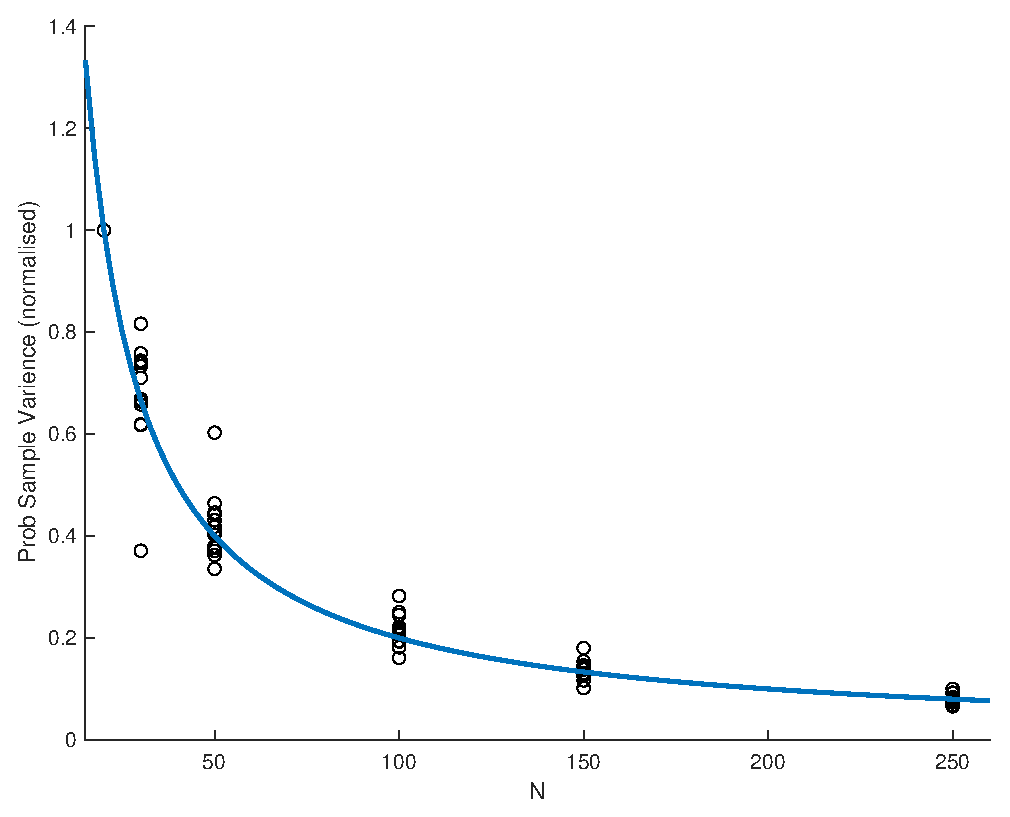
\includegraphics[width=12cm]{Image_3}
\caption{Sample variance of $\p(\mu_{k}>\theta|\y)$ for different $N$}\label{fg:3}
\end{figure}
Notice how both sample variances decay like $1/N$. This is a direct consequence of the Central Limit Theorem. It states that if $X_{i}\sim X$ are i.i.d and $\Var(X)<\infty$, then
\begin{equation}
\frac{1}{N}\sum_{i=1}^{N}X_{i}-\E(X)\xrightarrow{d}\text{N}\left(0,\frac{\Var(X)}{N}\right)
\end{equation}
in the limit as $N\rightarrow \infty$. We know that the sample variance of any i.i.d random variables converges almost surely to the true variance. Since the $X_{i}^{2}$ are uniformly integrable, then
\begin{equation}
\Var\left(\frac{\sum_{i}^{N}\left(X_{i}-\bar{X}\right)^{2}}{N-1}\right)\rightarrow\frac{\Var(X)}{N}
\end{equation}
asymptotically. This is exactly what we see in the two above figures; that as $N$ increases, the variation from the normalised hyperbola shrinks, with all data points practically lying on it at $N=250$.

\subsection*{\centering Question 7}
Sample variances were calculated by \nameref{cd:6}, referenced on page \pageref{cd:6}, with $N=30$, while $M=0,10,100$.  The value for $N$ was chosen deliberately small to highlight any changes in the distributions for small $M$. The simulations were repeated 500 times as before, and the results are tabulated in Table \ref{tb:4} below.

\begin{table}[H]
\centering
\begin{tabular}{c|ccc|ccc|}
\cline{2-7}
 & \multicolumn{3}{c}{$\mu_{k}$} \vline &  \multicolumn{3}{c}{$\p(\mu_{k}>\theta|\y)$}\vline \\ \cline{2-7}
$k$&$M=0$&$M=10$&$M=100$ & $M=0$ & $M=10$ & $M=100$\\ \hline
1 & 1.843564 & 2.237448 & 1.939471 & 1.081051e-4 & 1.182632e-4 & 1.569183e-4\\ 
2 & 0.4648628 & 0.4351083 & 0.4309788 & 3.686212e-3 & 3.447980e-3 & 3.992411e-3\\ 
3 & 0.6294533 & 0.7317089 & 0.6772295 & 2.928572e-3 & 2.954687e-3 & 3.086511e-3\\ 
4 & 0.6383631 & 0.7017769 & 0.6644687 & 4.627673e-3 & 4.874081e-3 & 4.215626e-3\\ 
5 & 0.2314946 & 0.1679683 & 0.2017004 & 3.287063e-4 & 2.038922e-4 & 2.483367e-4\\ 
6 & 2.331541 & 2.60194 & 2.796847 & 1.832304e-3 & 1.972389e-3 & 1.696811e-3\\ 
7 & 0.7538931 & 0.7933827 & 0.8928876 & 3.805348e-3 & 3.677091e-3 & 4.001117e-3\\ 
8 & 0.2473297 & 0.2971523 & 0.2557318 & 5.900512e-4 & 5.645557e-4 & 5.807659e-4\\ 
9 & 0.8379703 & 0.9233271 & 0.9659404 & 5.199091e-3 & 5.755350e-3 & 5.377025e-3\\ 
10 & 0.6053968 & 0.6235268 & 0.7439646 & 5.815631e-5 & 1.014072e-4 & 1.624360e-4\\ 
11 & 0.2069356 & 0.1995997 & 0.1818190 & 8.819906e-4 & 7.993943e-4 & 8.766466e-4\\ 
12 & 0.9143364 & 0.9594655 & 0.9342799 & 6.825206e-3 & 6.413231e-3 & 6.973787e-3\\ 
13 & 0.9178443 & 0.8146838 & 0.8955065 & 1.961630e-3 & 1.876802e-3 & 1.898352e-3\\ 
14 & 0.2940941 & 0.3144930 & 0.2827326 & 2.813431e-3 & 2.648746e-3 & 2.713315e-3\\ \hline
\end{tabular}
\caption{Sample variance in $\mu_{k}$ and $\p(\mu_{k}>\theta|\y)$ for different $M$}\label{tb:4}
\end{table}
There is very little change in the variance for $\mu_{k}$, suggesting that the distribution settles very quickly. This was intended, since the starting value $\x^{0}$ was chosen to be as close to the posterior distribution as possible (with no prior knowledge of $\y$). \\
The variance in $\p(\mu_{k}>\theta|\y)$ is also largely unaffected by the value of $M$ with a few sporadic large deviations. These can be ignored, since the method used to calculate $\p(\mu_{k}>\theta|\y)$ does not depend continuously on the values of $\mu_{k}$ and $\theta$. Thus, when $N$ is small,  the values calculated in different simulations can change by 'large' (discontinuous) amounts.

\subsection*{\centering Question 8}
The chain was run independently 500 times using a variety of starting states when $N=30$ and $M=70,0$. The sample means and variances of $\mu_{k}$ were calculated, as well as the distance (2-norm) between these vectors and the ones in Tables \ref{tb:1} and \ref{tb:4} respectively (in particular the calculated mean and $M=100$ variance of $\mu_{k}$). These norms are designed to indicate if the two distributions are similar by checking if the sample means and variances are close to the ones previously in the project. For the sake of notation, let $m_{M}$ denote the norm in the difference of means and $v_{M}$ likewise for the variance when the value $M$ is used. Also let $\mu_{k}^{(i)}$ denote the state $x_{k}^{i}$, $\sigma^{(i)}_{k}=x^{i}_{K+k}$ and $\theta^{(i)}=x^{i}_{2K+1}$. The following data tabulated in Table \ref{tb:5} was produced by \nameref{cd:6}.
\begin{table}[H]
\centering
\begin{tabular}{c|cccc}
Starting State & $m_{70}$ & $v_{70}$ & $m_{0}$ & $v_{0}$\\ \hline 
$\mu^{(0)}_{k}=60, \sigma^{(0)}_{k}=100, \theta^{(0)}=60$ &0.97288 & 0.53985 & 1.1936 & 0.64422\\ \hline
$\mu^{(0)}_{k}=1000, \sigma^{(0)}_{k}=0.001, \theta^{(0)}=1000$ & 0.93635 & 0.71239 & 0.87688 & 0.44730\\ \hline
$\mu^{(0)}_{k}=-500, \sigma^{(0)}_{k}=500, \theta^{(0)}=-500$ & 1.0400 & 0.67274 & 703.40 & 467.64\\
\hline
$\mu^{(0)}_{k}=-500, \sigma^{(0)}_{k}=500, \theta^{(0)}=60$ & 0.95777 & 0.62181 & 1.6842 & 0.78523\\
\end{tabular}
\caption{Effect of different starting states on MCMC}\label{tb:5}
\end{table}
We see that columns 2 and 3 match regardless of the starting state, confirming that the chain tends to the posterior distribution regardless of the starting distribution. Secondly notice that for our original starting state, $m_{0}\approx m_{70}$ and $v_{0}\approx v_{70}$, matching with the conclusion of Question 7 that in this case the posterior settles very quickly. However the values of $m_{0}$ and $v_{0}$ vary largely for different starting states, and this will be discussed in greater detail below by considering the conditional distributions in Question 2.\\

Affects of varying $\mu_{k}^{(0)}$: the way the chain is set up means that varying $\mu_{k}^{(0)}$ has no effect, since the conditional distributions of $\mu_{k}|\bm{\mu},\bm{\sigma}^{2},\theta$ do not depend on $\mu^{(0)}_{k}$. Therefore these parameters can be ignored\par
Affects of varying $\sigma^{(0)}_{k}$: if $\sigma^{(0)}_{k}$ is chosen to be very large, then $\mu_{k}^{(1)}$ is centred around $\theta^{(0)}$. Therefore if $\theta^{(0)}$ is chosen to be far away from the true expectation of $\mu_{k}$, then there will be a large error. This error will also cause the distribution of $\sigma^{(1)}_{k}$ to become shifted, and will cause a (partial) error in the value of $\theta^{(1)}$, but this is less important, since we average over the values of $\mu_{k}$. Therefore we expect slow convergence to the posterior (consistent with the above). Conversely if $\sigma^{(0)}_{k}$ is chosen to be small, then $\mu^{(1)}_{k}$ is distributed as a sharp spike around the value $\sum_{t=1}^{T}y_{kt}/T$. This is very close to the mean of the posterior distribution, and so there is almost no error, and thus $\theta^{(1)}$ and $\sigma^{(1)}_{k}$ will be distributed correctly as well. This causes the distribution to settle very quickly. (consistent with the above). \par
Affects of varying $\theta^{(0)}$: We've seen that the value of $\theta^{(0)}$ only has an effect on the chain if $\sigma_{k}^{(0)}$ is chosen to be large. If this is the case then we require $\theta^{(0)}$ to be a reasonable estimate for the average of all $\mu_{k}$. This way any individual $\mu_{k}$ will (hopefully) not be too far away from it's true mean, and hence the distribution settle relatively quickly. Compare the last two starting states in Table \ref{tb:5}. The results confirm exactly this point; that when $\theta^{(0)}$ is near the average the posterior settles far quicker.\\

We conclude that the value of $M$ is only important when the starting state has $\sigma^{(0)}$ chosen to be large and $\theta^{(0)}$ chosen far away from the average. 

\pagebreak
\section*{\centering Code}
\subsection*{\centering Gibbs Sampler}\label{cd:Gibbs}
\begin{verbatim}
digits(8)
Data={"Team","2024","2023","2022","2021","2020"
"Arsnal",83,90,78,87,81
"Asten Villa",47,56,45,50,60
"Blackborn Rovers",42,44,60,46,56
"Boltin Wandrers",58,53,44,40,60
"Charlston Athletic",46,53,49,44,45
"Chelsea Buns",95,79,67,64,71
"Evraton",61,39,59,43,46
"Fullem",44,52,48,44,53
"Livurpule",58,60,64,80,54
"Manchester Ununited",77,75,83,77,70
"Middlesbro",55,48,49,45,51
"Newcassel Divided",44,56,69,71,64
"Slothampton",32,47,52,45,55
"Tottenham Coldspur",52,45,50,50,59};
K=size(Data,1)-1;
T=size(Data,2)-1;

sigma_0=10;
alpha_0=10^-5;
beta_0=10^-3;
mu_0=60;
tau_0=20;

StartVal=zeros(2*K+1,1);
StartVal(1:2*K+1)=60;
StartVal(K+1:2*K)=100;

N=5;
tic
Sim=Gibbs(Data,sigma_0,alpha_0,beta_0,mu_0,tau_0,N,StartVal)
latex(sym(vpa(Sim)))
toc

function Simulations = Gibbs(Data,sigma_0,alpha_0,beta_0,mu_0,tau_0,N,StartVal)
K=size(Data,1)-1;
T=size(Data,2)-1;

%Standardizes parameters
sigma_0=sigma_0^2;
tau_0=tau_0^2;

Simulations=zeros(2*K+1,N+1);
Simulations(:,1)=StartVal;
Counter=2;

while Counter<=N+1
    lineLength = fprintf('%.1f%% complete',Counter*100/N);
    SubCounter=1;
    while SubCounter<=2*K+1
        if SubCounter<=K
            %   SIMULATING MU PARAMETERS
            sigma_k=Simulations(SubCounter+K,Counter-1);
            sumData=sum([Data{SubCounter+1,2:T+1}]);
            theta=Simulations(2*K+1,Counter-1);
            Mean=(sigma_k^(-1)*sumData+theta*sigma_0^(-1))/(T*sigma_k^(-1)+sigma_0^(-1));
            Var=1/(T*sigma_k^(-1)+sigma_0^(-1));
            Simulations(SubCounter,Counter)=normrnd(Mean,sqrt(Var));
        elseif SubCounter<=2*K
            %   SIMULATING SIGMA PARAMETERS
            sumData=sum(([Data{SubCounter-K+1,2:T+1}]-Simulations(SubCounter-K,Counter)).^2);
            Mean=alpha_0+T/2;
            Var=beta_0+sumData/2;
            Simulations(SubCounter,Counter)=(gamrnd(Mean,1/Var))^-1;
        else
            %   SIMULATING THETA PARAMETER
            sumData=sum(Simulations(1:K,Counter));
            Mean=(sigma_0^-1*sumData+mu_0*tau_0^-1)/(K*sigma_0^-1+tau_0^-1);
            Var=1/(K*sigma_0^-1+tau_0^-1);
            Simulations(SubCounter,Counter)=normrnd(Mean,sqrt(Var));
        end
        SubCounter=SubCounter+1;
    end
    fprintf(repmat('\b',1,lineLength))
    Counter=Counter+1;
end
end
\end{verbatim}

\pagebreak
\subsection*{\centering Code 4}\label{cd:3}
\begin{verbatim}
digits(8)

sigma_0=10;
alpha_0=10^-5;
beta_0=10^-3;
mu_0=60;
tau_0=20;

StartVal=zeros(2*K+1,1);
StartVal(1:2*K+1)=60;
StartVal(K+1:2*K)=100;

tic
N=250;
Sim=Gibbs(Data,sigma_0,alpha_0,beta_0,mu_0,tau_0,N,StartVal);
toc

PosteriorMean=sum(Sim(:,2:end),2)./N;
EstimatedMeans=zeros(K,4);
EstimatedMeans(:,1)=PosteriorMean(1:K);
EstimatedMeans(:,3)=PosteriorMean(K+1:2*K);
EstimatedMeans(:,2)=sum(cell2mat(Data(2:K+1,2:T+1)),2)/T;
EstimatedMeans(:,4)=sum((cell2mat(Data(2:K+1,2:T+1))-EstimatedMeans(:,2)).^2,2)/(T-1);
sum(EstimatedMeans(:,1))

disp(EstimatedMeans)
latex(sym(vpa(EstimatedMeans)))

thetaData=Sim(end,2:end);
mid=sum(thetaData)/N

XLower=min(thetaData)-2;
XHigher=max(thetaData)+2;

h=figure;
histogram(thetaData,'Normalization','pdf')
xlabel('\theta')
ylabel('Frequency Density')
print(h,'Image_1','-depsc')

\end{verbatim}

\pagebreak
\subsection*{\centering Code 5}\label{cd:4}
\begin{verbatim}
digits(8)

sigma_0=10;
alpha_0=10^-5;
beta_0=10^-3;
mu_0=60;
tau_0=20;

List=[20,30,50,100,150,250];
NCounter=1;
MeanProb=zeros(K,size(List,2));
MeanMu=zeros(K,size(List,2));
VarProb=zeros(K,size(List,2));
VarMu=zeros(K,size(List,2));

while NCounter<=size(List,2)
N=List(1,NCounter);
Number_of_Runs=500;

Prob=zeros(K,Number_of_Runs);
Mu=zeros(K,Number_of_Runs);

SuperCounter=1;
while SuperCounter<=Number_of_Runs

LineLength=fprintf('List: %d, Run: %.1f%% complete',N,SuperCounter*100/Number_of_Runs);
Sim=Gibbs(Data,sigma_0,alpha_0,beta_0,mu_0,tau_0,N);

Counter=2;
Carry=zeros(K,1);
while Counter<=N+1
    SubCounter=1;
    while SubCounter<=K
        if Sim(SubCounter,Counter)>Sim(2*K+1,Counter)
            Carry(SubCounter,1)=Carry(SubCounter,1)+1;
        end
        SubCounter=SubCounter+1;
    end
    Counter=Counter+1;
end
Prob(:,SuperCounter)=Carry/N;
Carry=sum(Sim,2);
Mu(:,SuperCounter)=Carry(1:K,1)/N;
fprintf(repmat('\b',1,LineLength))
SuperCounter=SuperCounter+1;
end

MeanProb(:,NCounter)=sum(Prob,2)/Number_of_Runs;
VarProb(:,NCounter)=sum((Prob-MeanProb(:,NCounter)).^2,2)/(Number_of_Runs-1);
MeanMu(:,NCounter)=sum(Mu,2)/Number_of_Runs;
VarMu(:,NCounter)=sum((Mu-MeanMu(:,NCounter)).^2,2)/(Number_of_Runs-1);
NCounter=NCounter+1;
end
disp(MeanMu)
disp(VarMu)
disp(MeanProb)
disp(VarProb)

figure
Counter=1;
while Counter<=K
    scatter(List,VarMu(Counter,:)/VarMu(Counter,1),'k')
    hold on
    Counter=Counter+1;
end
x=linspace(List(1,1)-5,List(1,end)+10);
y=List(1,1)./x;
plot(x,y,'LineWidth',2)
xlim([List(1,1)-5,List(1,end)+10])
xlabel('N')
ylabel('\mu Sample Varience (normalised)')
print('Image_2','-depsc')

figure
Counter=1;
while Counter<=K
    scatter(List,VarProb(Counter,:)/VarProb(Counter,1),'k')
    hold on
    Counter=Counter+1;
end
x=linspace(List(1,1)-5,List(1,end)+10);
y=List(1,1)./x;
plot(x,y,'LineWidth',2)
xlim([List(1,1)-5,List(1,end)+10])
xlabel('N')
ylabel('Prob Sample Varience (normalised)')
print('Image_3','-depsc')

\end{verbatim}
\pagebreak

 \subsection*{\centering Code 7}\label{cd:6}
 \begin{verbatim}
digits(8)
K=size(Data,1)-1;
T=size(Data,2)-1;

sigma_0=10;
alpha_0=10^-5;
beta_0=10^-3;
mu_0=60;
tau_0=20;

CalculatedMean=[81.4968825139968;52.1355802069355;50.672260968429;52.5080817745987;...
    48.1389564329937;69.784992226184;51.6374396731938;48.7565228578938;...
    62.2933104774652;74.386133868267;49.8382175215858;59.9520363668573;...
    48.2862648696441;51.5355709368392];
CalculatedVar=[1.9394709;0.43097878;0.67722952;0.66446875;0.20170042;2.7968475;0.89288769;...
    0.25573182;0.96594047;0.74396463;0.18181906;0.93427989;0.89550653;0.2827326];

StartingValue=zeros(2*K+1,1);
StartingValue(1:2*K+1)=60;
StartingValue(K+1:2*K)=100;
StartingValue(2*K+1)=60;

List=[0,70];
N=30;

NCounter=1;
MeanProb=zeros(K,size(List,2));
MeanMu=zeros(K,size(List,2));
VarProb=zeros(K,size(List,2));
VarMu=zeros(K,size(List,2));

while NCounter<=size(List,2)
M=List(1,NCounter);
Number_of_Runs=500;

Prob=zeros(K,Number_of_Runs);
Mu=zeros(K,Number_of_Runs);

SuperCounter=1;
while SuperCounter<=Number_of_Runs

LineLength=fprintf('List: %d, Run: %.1f%% complete',M+N,SuperCounter*100/Number_of_Runs);
Sim=Gibbs(Data,sigma_0,alpha_0,beta_0,mu_0,tau_0,M+N,StartingValue);

Counter=2+M;
Carry=zeros(K,1);
while Counter<=M+N+1
    SubCounter=1;
    while SubCounter<=K
        if Sim(SubCounter,Counter)>Sim(2*K+1,Counter)
            Carry(SubCounter,1)=Carry(SubCounter,1)+1;
        end
        SubCounter=SubCounter+1;
    end
    Counter=Counter+1;
end
Prob(:,SuperCounter)=Carry/N;
Carry=sum(Sim(:,M+2:M+N+1),2);
Mu(:,SuperCounter)=Carry(1:K,1)/N;
fprintf(repmat('\b',1,LineLength))
SuperCounter=SuperCounter+1;
end

MeanProb(:,NCounter)=sum(Prob,2)/Number_of_Runs;
VarProb(:,NCounter)=sum((Prob-MeanProb(:,NCounter)).^2,2)/(Number_of_Runs-1);
MeanMu(:,NCounter)=sum(Mu,2)/Number_of_Runs;
VarMu(:,NCounter)=sum((Mu-MeanMu(:,NCounter)).^2,2)/(Number_of_Runs-1);
NCounter=NCounter+1;
end
disp(MeanMu)
disp(VarMu)
latex(sym(vpa(VarMu)))

Norms=[List;vecnorm(MeanMu-CalculatedMean);vecnorm(VarMu-CalculatedVar)];
disp(Norms)
latex(sym(vpa(Norms)))

disp(MeanProb)
disp(VarProb)
latex(sym(vpa(VarProb)))

\end{verbatim}
\end{document}
